\documentclass[11pt]{article}
\usepackage{graphicx}
\usepackage{caption}
\usepackage{chngcntr}
\usepackage[section]{placeins} % subsections
\usepackage[round, sort, numbers]{natbib}
\usepackage{makecell}
\usepackage{url}
\counterwithin{figure}{section}
\captionsetup[figure]{slc=off}
\usepackage[left=2cm, right=2cm, top=2cm, bottom=2cm]{geometry} % geometry of page
\setcitestyle{square} % square referencing style
\usepackage[fleqn]{amsmath} % for maths
\usepackage{subfig}
\setlength{\parindent}{0pt} % no indents on new paragraphs
\graphicspath{{Code/Analysis/Figures/}}

\begin{document}
\begin{titlepage}
    \begin{center}
        \vspace*{1cm}
        \Huge
        \textbf{Robotics} \\
        \vspace{0.5cm}
        \LARGE
        \vspace{1.5cm}
        \textbf{G. Sheppard, D. Thomas, J. Doering, J. Matthews, C. Li} \\
        \vfill
        \vspace{0.8cm}
        \Large
        University of Birmingham\\
        Physics and Astronomy Department\\
    \end{center}
\end{titlepage}

\tableofcontents

\section{Abstract}
Wow look at \ref{angleplot}. \cite{Bae2006}.

\section{Connecting}
\subsection{NAO}
David: you know what to write
\subsection{Hinge Encoders}
George: difficulties for connecting on own computer, procedure for connecting on lab pc, need for libraries in right place etc, link to wiki in appendix

\section{Creating Algorithms}
---------------------------------------------------------George Sheppard---------------------------------------------------------

The creation of each individual algorithm required a substantial amount of common code, for example: connecting to NAO, collecting angle values from both sets of hinge encoders, and processing these data. For this reason the code was structured such that new algorithms could be freely created that each integrated with the base code. This base code collected all values relating to the swinging motion, passed these values through an algorithm, stored these values, and fixed the cycle rate. Additionally, due to this structure, mock classes for NAO and the hinge encoders were created such that this interface could be developed away from the lab, and a testing setup was added such that a user would be able to re-run previous recorded data and plot how their algorithm reacted to that scenario.\\

With this base structure in place, creating an algorithm involved one function that took a set of values, and decided how to react to them, the algorithm also had access to all past data to help in decision making. As these algorithms were defined in the same way, it is easy to switch between different algorithms mid swing, such that the motion of NAO could be more stringently controlled. For example NAO could be told to increase to $30^o$, then maintain this amplitude for $10s$, and then finally decrease back down to $0^o$.  This base structure also included the pre-defined positions for NAO, such that switching positions could be done by just calling a function with the name of the position.

\section{Simple Pendulum}
\subsection{Start Up}
James: talk about two positions defined for the motion, idea behind the algorithm, how it links into the next algorithm that increases amplitude, results, why is it tricky to start off like this (have to predict when to swing very well sort of stuff), if multiple algorithms created do for each

\subsection{Increasing and Decreasing Amplitude}
\subsubsection{Parametric Pumping}
Jon: Talk about two extra positions defined for this motion, the idea behind the algorithm, results try to fit to exponential curve to see if it multiplies amplitude by fixed fraction like worksheet showed, any limitations, were two positions just different in vertical centre of mass or did horizontal distance change too
\subsubsection{Torque Method TODO: BETTER NAME FOR THIS}
George/David: Say used previous defined positions, different methods for each algorithm (quarter period, theory team calculation of max angle), results for each, try to fit maximum amplitude peaks to linear to see if proportional to distance rocked or not, how results varied on different parameters such as if he swings before peak, during, or after, limitations to each method

\subsection{Maintaining Amplitude}
Chenglong: different subsubsection for each method you used, first outline the idea behind each algorithm, then show the results for each, compare and contrast after you have shown results for each, which was easiest to code, had the finest control over the angle (calculate variance on the maximum amplitude of the swing), which is most efficient, anything else you decide is good

\subsubsection{Conclusion}
Everyone: Think this should just be how to improve, any difficulties of the setup, which is the best method and why etc

\section{Triple Pendulum}

\begin{figure}[!htb]
    \centering
    \captionbox
         {Angleplot.\label{angleplot}}
         {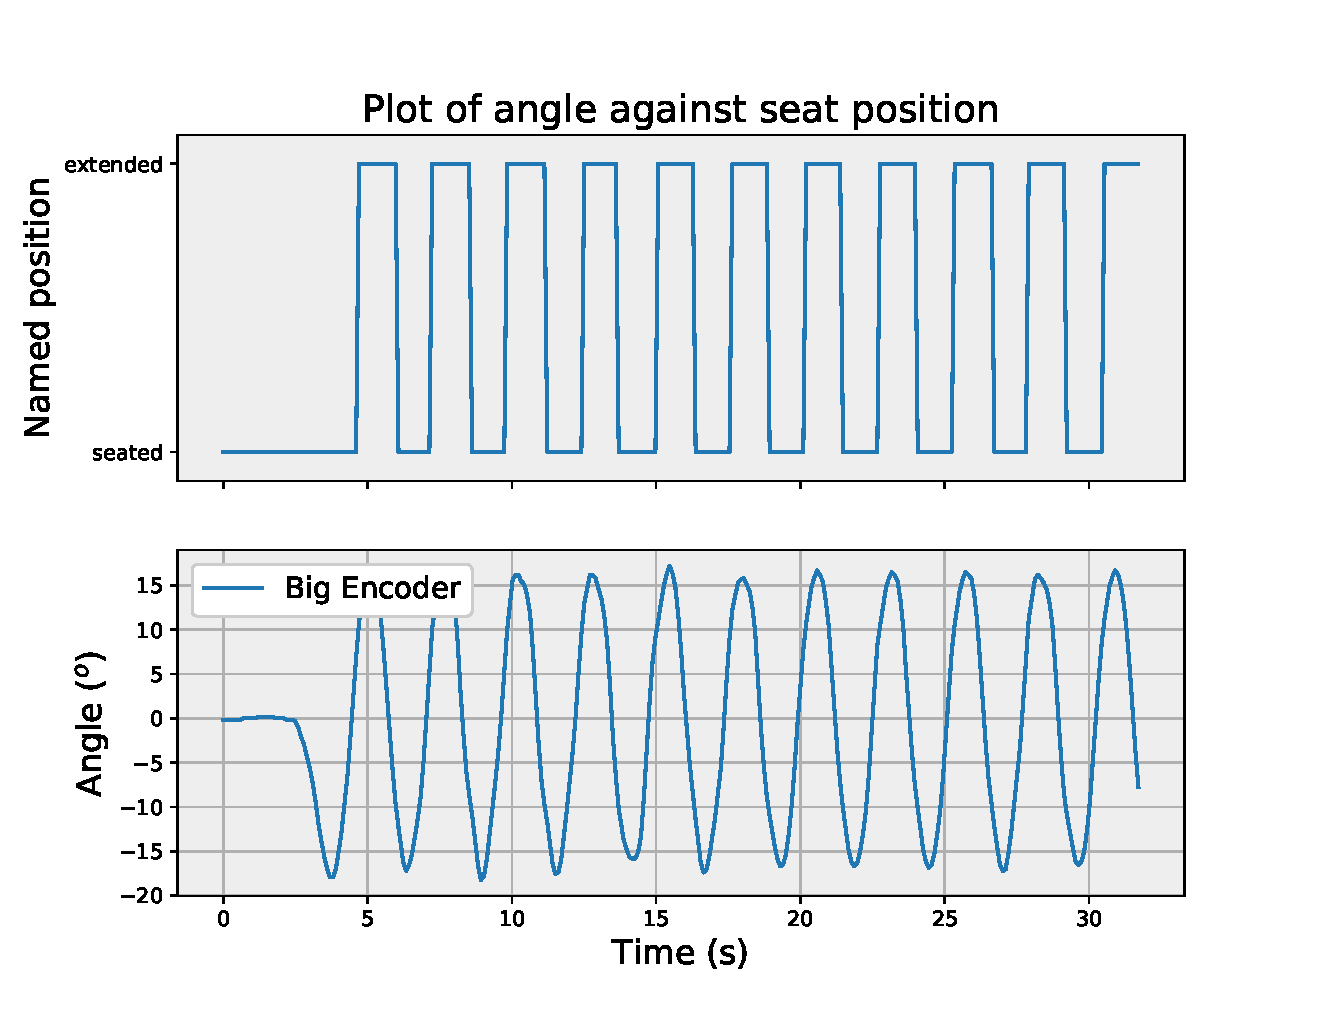
\includegraphics[width=1.0\textwidth]{AnglePlot15-02-201913:29:23}}
\end{figure}

\appendix
\section{Appendix}
\subsection{Wiki}
---------------------------------------------------------George Sheppard---------------------------------------------------------
Throughout this project, there were a large amount of issues found when trying to connect to: NAO, Webots, and the hinge encoders etc. For this reason a wiki was created to document how to set everything up correctly. This wiki is available at: https://github.com/GeorgeSheppard/Robotics. Alongside this wiki is the final code, including how to use it, the report, and any analysis files used to create plots. Feel free to clone this repository and add to it such that there remains a comprehensive guide for each year.

\bibliographystyle{ieeetr}
\bibliography{References}
\end{document}